% calibration of heo /mnt/backup/safe-with-time/torben/safed/y2009/0512
% measurement double plane /mnt/backup/safe-with-time/torben/safed/0525
% talk /mnt/backup/safe-with-time/torben/safed/0321/talk
\chapter{Holographic approach to spatio-angular illumination}
\begin{summary}
  Here we present an alternative system for spatio-angular control. It
  is based on a single phase-only LCoS. This simplifies electronic
  synchronization.
\end{summary}

\section{Introduction}
In this part we describe a very different approach that simplifies the
setup considerably.

\begin{figure}[!hbt]
  \centering
  \input{holo-setup3.eps_tex}
  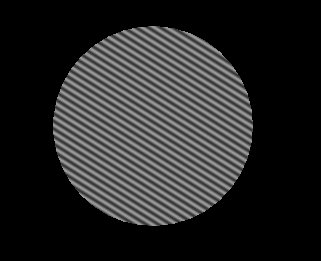
\includegraphics[height=1cm]{hologram-disk}
  \caption{Schematic of the holographic spatio-angular microscope. A
    phase only LCoS in the intermediate image plane displays a grating
    and steers the first order into the back focal plane of the
    objective. Period and orientation define the angle of the
    illumination in the sample. Shape and contrast of the grating
    define the illuminated area and intensity of the illumination.}
  \label{fig:holo-setup3}
\end{figure}

\figref{fig:holo-setup3} shows a schematic of the setup. The main
component is a phase-only spatial light modulator in the intermediate
image plane. When nothing is displayed on the spatial light modulator,
it will reflect the Gaussian laser beam into a beam dump, so that
the light cannot enter the tube lens.

\section{Description of the holographic method}
The spatial light modulator is then programmed to display a phase
grating.  The direction and periodicity of a grating can be chosen
such that the first order is steered into any position on the back
focal plane. In the sketch the grating directs the first order into
the periphery of the back focal plane. Therefore the specimen will be
illuminated by light under a steep angle (not visible in
\figref{fig:holo-setup3} due to exaggerated focal length of
objective).

Decreasing the size of the grating will decrease the size of the
illuminated area in the object. Note that a grating of very small size
gives rise to a wide first order in the back focal plane, limiting the
possible angular control.
\subsection{Description of the experimental setup}
We use a HEO 1080 P High-Resolution LCOS Phase Only Spatial Light
Modulator (Holoeye, Berlin, Germany) to control the phase in the
intermediate plane. The light source is a \unit[473]{nm} DPSS diode
laser. It is coupled into a polarization maintaining fibre and
collimated by a \unit[150]{mm} lens with \unit[50]{mm} diameter.

The tube lens has \unit[300]{mm} diameter and the objective is a
$63\times/1.4$ with oil immersion.  For aligning the optical system a
sequence of device filling gratings was displayed at 60Hz. The
parameters of the grating were chosen such that the first order
describes a circle in the back focal plane.

\subsection{Description of the sample}
To show that the illumination angle of the light was indeed adjustable
a test sample was constructed. A slide and a cover slip were coated
with a thin fluorescent plane (see \figref{fig:holo-setup3}). The air
gap between the two fluorescent planes was approximately five
micrometres thick.

Imaging the fluorophore plane on the slide resulted in a haze of
background fluorescence stemming from the cover slip (see
\figref{fig:holo-meas}). Changing the illumination angle resulted in a
rotation of this haze as one would expect.
\begin{figure}
  \centering
  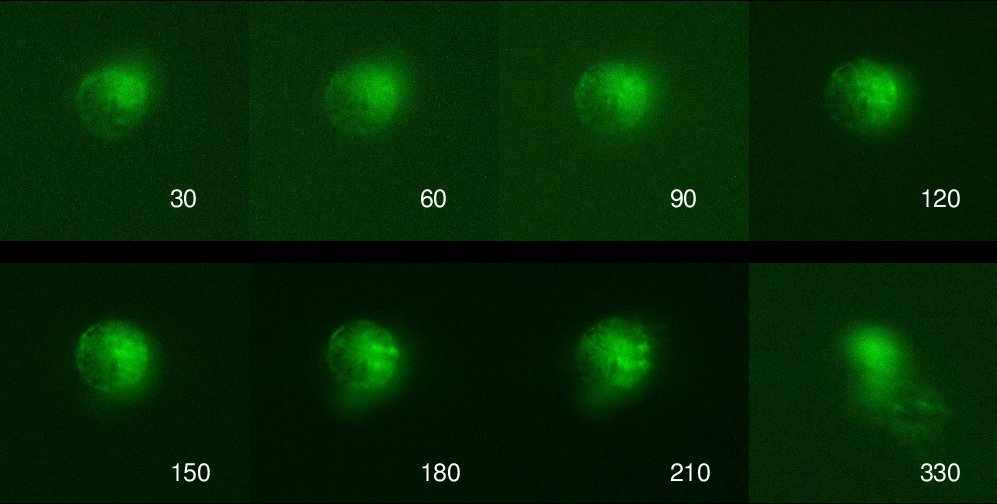
\includegraphics[width=12cm]{haze}
  \caption{Widefield images of a sample of two parallel fluorescent
    planes with varying azimuth angle of the illumination (numbers in
    in degree). One of the fluorescent planes is in focus, the other
    is imaged as an unsharp haze.}
  \label{fig:holo-meas}
\end{figure}

\section{ Characterization of the phase-only spatial light modulator}
\begin{summary}
  Here we measure the correspondence between displayed gray values and
  resulting phase difference on the Holoeye HEO 1080P spatial light
  modulator.
\end{summary}
We use a similar setup as given in the manual \citep{Holoeye2006}.
\begin{figure}[!hbt]
  \centering
  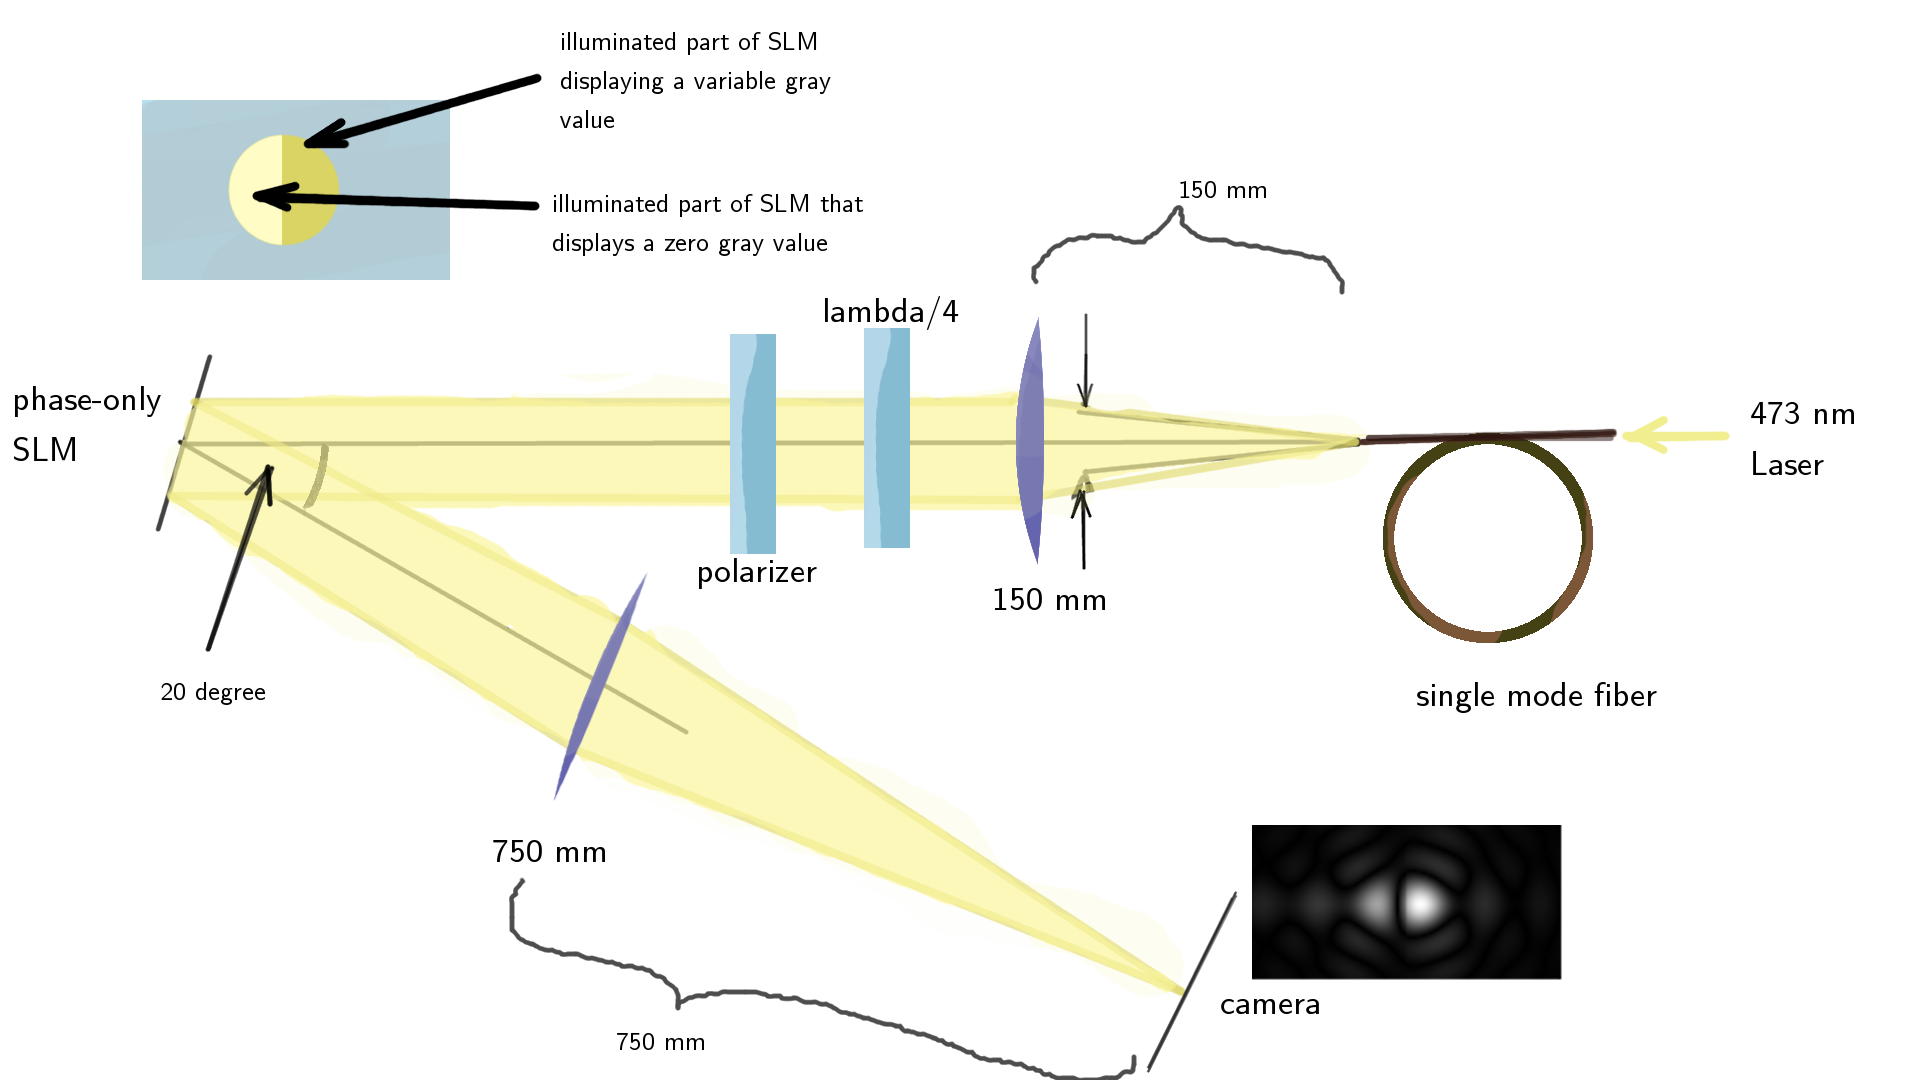
\includegraphics[width=16cm]{sketch}
  \caption{Setup for calibrating the transfer function of the phase
    SLM. We will establish, which gray values correspond to what phase
    delay. The light from a polarization maintaining single mode fibre
    is circularly polarized by a $\lambda/4-$plate and a polarizer is
    then used to select the optimum polarization direction. The
    Fraunhofer diffraction pattern of light, which has been reflected
    from the device, is captured with a fast camera. (The display's
    cable would come out at the top, perpendicular to the paper
    plane.)}
  \label{fig:holo-calib}
\end{figure}
The SLM is illuminated with a parallel linearly polarized wave
front. The plane of vibration of the electric field is in the paper
plane.

The SLM displays two vertical bars. The left bar shows black (0) and
the upper bar displays a gray value that is varied for the
measurement.  The beam has a circular shape and a (sufficiently)
constant intensity distribution. The beam is centred on the line
between the two bars of different phase. 
\subsection{Numerical simulation}
The minima of the diffraction pattern in the Fourier plane (on the
camera) move proportional to the phase difference between the two
parts of the display (see \figref{fig:holo-theory}).
\begin{figure}[!hbt]
  \centering
  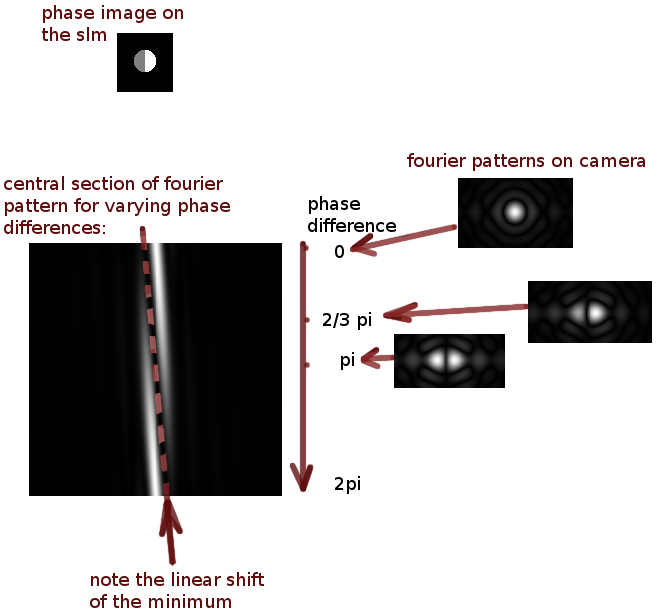
\includegraphics[width=12cm]{theory}
  \caption{Theoretical simulation of the Fraunhofer diffraction
    pattern for varying phase difference between the two sides of the
    display.}
  \label{fig:holo-theory}
\end{figure}
For the simulation we calculated the Fourier transform of a phase
image with a geometry as shown in the top left image in
\figref{fig:holo-theory}.  The three images on the right show the
Fraunhofer diffraction patterns of this (reflective) phase image for
three different values of the phase difference between the half
circles. The position of the minimum changes proportionally to the
phase difference. Therefore we can measure the position of the extrema
to determine the relationship between gray value and phase difference
(the transfer function of the device).

\subsection{Measurement}
The result of this measurement is shown in the top of
\figref{fig:holo-transfer}
(horizontal section through centre of
the Fourier pattern against gray value)
\begin{figure}[!hbt]
  \centering
  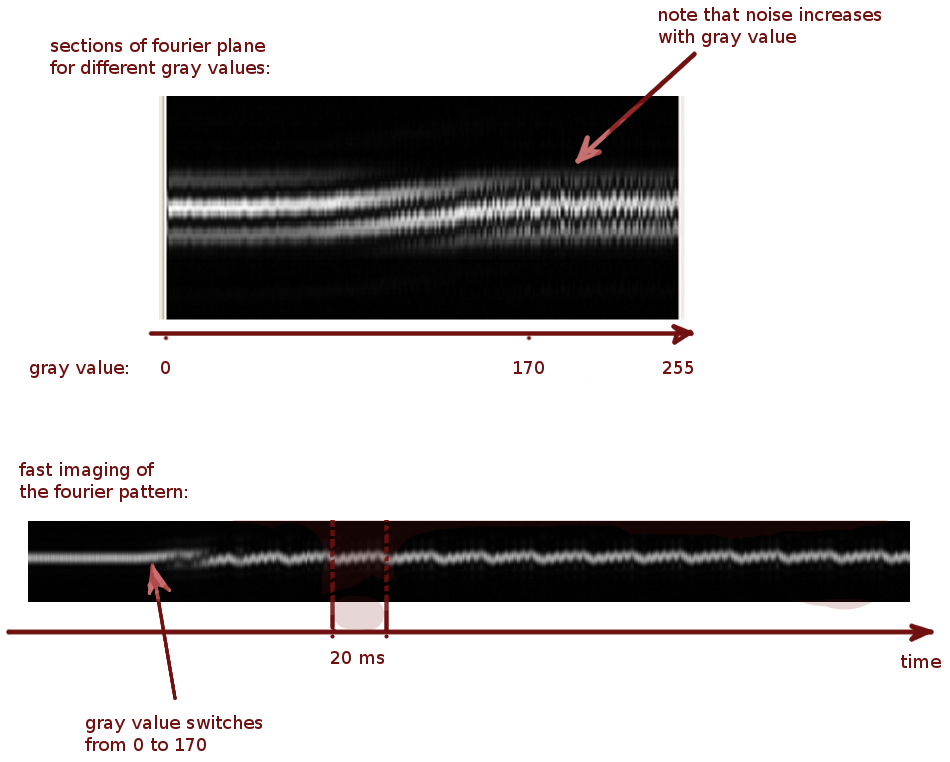
\includegraphics[width=16cm]{measure}
  \caption{{\bf top:} horizontal sections through the Fraunhofer
    diffraction pattern on the camera are plotted as columns. The
    displayed gray value is plotted as the x-axis. {\bf bottom:} Time
    variation of the phase, when a constant value of 170 is shown. The
    phase fluctuates considerably.}
  \label{fig:holo-transfer}
\end{figure}
The measurement shows that a phase difference of $2\pi$ can be induced
for a sufficiently high gray value. However we observe significant
noise for the phase measurements.  There are jumps in the data that
amount to several 10 gray values. 

To analyze this effect further a fast camera (mvBlueFox 102G, 2400 Hz,
$200\times4$ region of interest, $\unit[ 6]{\mu m}$ pixel size) was
used to image the Fourier pattern with a high time resolution.  The
bottom image in \figref{fig:holo-transfer} displays 1000 horizontal
line sections over the centre of the Fourier plane. In the beginning,
both half circles were displaying a gray value of zero. Then the right
half circle was suddenly set to 170. The transient occurs quite fast
but then there is a waveform with 5 peaks that repeats with 50 Hz (the
refresh rate of the display).

The measurement suggests that the phase difference of the Holoeye SLM
is varying significantly over time. In order to improve the
performance for displaying computer generated holograms we could
trigger the laser only for a short time before a new frame will be
displayed.

From other experiments we know that there is also cross talk between
the pixels, i.e. if a fine grating is displayed, the displayed phase
contrast is lower than for a coarser grating.
\section{Conclusion}
With our prototype system we showed that it is possible to use the
phase-only SLM to achieve angular and spatial control of the
illumination. Further work would be necessary to optimize the grating
fine structure in order to direct more light is directed towards the
first order (blazing).

Compared to the MEMI system a lot less synchronization between devices
is necessary. However, this technique is only possible with coherent
illumination. Furthermore there is no inherent advantage in the
holographic method as light from dark areas is sent into a beam stop
and is lost as in the MEMI system.

It might be possible to build a system using a kinoform element (two
phase holograms in different positions). This would allow to redirect
light from dark areas into bright areas leading to a much more
efficient system. A different display device with less cross talk
and fluctuations would be advisable for this.

